\DiaryEntry{Graph Theory - Fundamentals}{2020-07-13}{Graphs}

\subsection{Basic Definitions}

A graph $G$ is an ordered pair of disjoint sets $(V,E)$, such that the edge set $E$ is a subset of $V^{(2)} = V \times V$, where $V$ denotes the set of vertices. An edge $\{x,y\}$ connects or joins two (end)vertices $x$ and $y$, which are also called adjacent or neighbouring vertices of $G$.

We call $G' = (V', E')$ a \emph{subgraph} of a graph $G$ if $V' \subset V$ and $E' \subset E$. If the subgraph contains all egdes of $E$ that have endpoints in $V'$, then it is called a \emph{spanning subgraph}.

The following Figure shows an example graph $G$ (left) along with the induced subgraph $G'$ (right) which was created by removing vertex $4$. Since $G'$ contains call edges from $G$ which have endpoints in $V'$, it is an induced subgraph.

\begin{figure}[H]
\centering
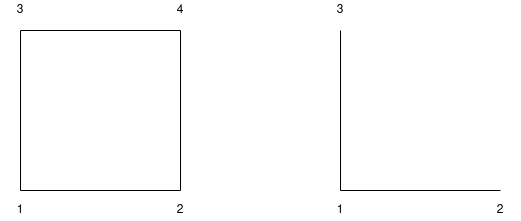
\includegraphics[scale=0.5]{images/graphs_03_01.png}
\end{figure}

We can construct new graphs from old ones by deleting or adding edges / vertices. If $W \subset V(G)$, then $G - W$ is the subgraph of $G$ obtained by deleting all vertices of $W'$ and all edges incident with them. In a similar spirit, if $E' \subset E$, then $G - E'$ is the subgraph obtained by deleting all edges of $E'$ and all associated vertices.

In the above example, $W = \{4\}$, therefore $V(G') = G - \{4\}$ and $E(G') = G - \{(2,4), (3,4)\}$.

In a similar spirit we can define addition of edges / vertices to a graph.

We finally define the \emph{complement} $\bar{G}$ of a graph $G = (V,E)$ as $\bar{G} = V, V \times V - E)$. Two vertices are adjacent in $\bar{G}$ if they are not adjacent in $G$.

The \emph{order} $|G|$ of a graph $G$ is defined as the number of its vertices, i.e. $|G| = |V(G)|$. The \emph{size} $e(G)$ of a graph $G$ is defined as the number of edges $e(G) = |E(G)|$. We denote by $G(n,m)$ a graph of order $n$ and size $m$.

The size of a graph $G$ with order $n$ is at least $0$ (the empty graph $E_n = \bar{K_n}$) and at most ${n} \choose {2} = \frac{n(n-1)}{2}$, which is the complete $n$-graph denoted by $K_n$. In this graph, every vertex is connected via an egde.

The set of vertices adjacent to a vertex $x \in G$ is called the \emph{neighbourhood}, $\Gamma(x)$. $x \sim y$ means that vertex $x$ is adjacent to vertex $y$; therefore $y \in \Gamma(x), x \in \Gamma(y), x \sim y, y \sim x$ are all equivalent, each of them meaning that $xy$ is an edge. The \emph{degree} $d(x)$ of a vertex $x$ is $d(x) = |\Gamma(x))|$. The minimal degree of a graph $G$ is denoted as $\delta(G)$, the maximum degree is denoted as $\Delta(G)$.

Since each edge has two endvertices, the sum of the degrees is twice the number of edges,

\be\label{eq:graph_03:01}
\sum_{i=1}^n d(x_i) = 2 e(G)
\ee

From this we conclude that the sum of degrees is even,

\bee
\sum_{i=1}^n d(x_i) \equiv 0 \mod 2
\eee

The sum of (two) even numbers is always even; however, only the sum of an even number of odd numbers is even (e.g. $1+3=4, 1+3+5+1 = 10$, but $1+3+1 = 5$). Therefore, the number of vertices with odd degree must be even. From the first sum we can obtain bounds for the minimum and maximum degree as follows,

\bee
\delta(G) \leq 2 e(G) / n, \quad \Delta (G) \geq 2e(G) / n
\eee


\subsection{Walks, Paths, etc}

If we move along a graph, several new definitions are required.

\begin{itemize}
\item A \emph{walk} $W$ in a graph $G$ is an alternating sequence of vertices and edges; e.g. $x_0, e_1, x_1, e_2, \ldots x_l$, where the edge $e_i = x_{i-1}x_i$.
\item A \emph{trail} is a walk if all edges are distinct.
\item A \emph{path} is a trail in which all vertices (and therefore also all edges) are distinct.
\item A \emph{circuit} is a non-empty trail in which the first and last vertices coincide.
\item A \emph{cycle} is a circuit of length larger $2$ and all vertices but $x_0=x_l$ are distinct from each other. We denote cycles of length $l$ with $C_l$ and call them $l$-cycles; in particular, $C_3$ is a triangle, $C_4$ is a quadrilateral, and $C_5$ is a pentagon.
\end{itemize}

We can also see a path $P$ as a graph itself, having the form

\bee
V(P) = \{x_0, x_1,\ldots,x_l\}, \quad E(P) = \{x_0 x_1, x_1 x_2, \ldots,x_{l-1} x_l\}
\eee

with $x_i \neq x_j, \forall i \neq j$. The vertices $x_0, x_l$ are denoted endvertices of $P$, and $l=e(P)$ is the length of the path. We call $P$ also a path from $x_0$ to $x_l$ or a $x_0 - x_l$-path.

The term \emph{independent} can be used with edges, vertices, and paths. A set of vertices is independent, if no two vertices are adjacent. Analogously, a set of edges is independent, when no two edges are adjacent; i.e. do not share a common vertex. In the example graph above, e.g. vertices $1$ and $4$ are independent; and edges $12$ and $34$ are independent. A set of paths is independent if for any two paths each vertex belonging to both paths is an endvertex to both. Thus, two paths $P_1$ and $P_2$ are independent $x-y$-paths, iff $V(P_1) \cap V(P_2) = \{x,y\}$; i.e. the two paths share only the startvertex and endvertex.

The graph in the following Figure has two cycles: $1-2-3$ and $1-4-5$; note that $1-2-3-1-4-5$ is \emph{not} a cycle as not all vertices (but $x_0$) are distinct. It is, however, a circuit.

\begin{figure}[H]
\centering
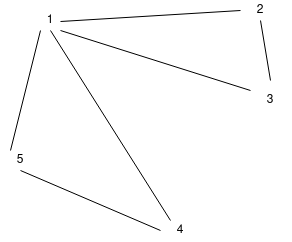
\includegraphics[scale=0.5]{images/graphs_03_02.png}
\end{figure}

We have Veblen's theorem regarding cycles.

\begin{theorem}
If a graph has even degree at each of its vertices, then it is possible to find a set of simple cycles that together cover each edge exactly once; i.e. the graph can be partitioned into a set of cycles. This holds true regarldess whether the graph is connected or not.
\end{theorem}

In the above Figure, the two cycles $1-2-3$ and $1-4-5$ cover each edge exactely once, showing the validity of Veblen's theorem. Had we another edge between vertices $3$ and $4$, we could not decompose the graph into edge disjoint cycles; however, in this case, vertices $3$ and $4$ would have odd degree.

\begin{proof}
  The graph is a union of edge disjoint cycles (and isolated vertices); each vertex is contained in $k$-cycles and therefore has degree $2k$ which is even.

  Suppose that every vertex has even degree and $e(g) > 0$. We want to find a cycle in $G$: Let $x_0 x_1 \ldots x_l$ be a path of maximal length $l$ in $G$. Since $x_0 x_1 \in E(G)$, we have $d(x_0) \geq 2$. But then $x_0$ has another neighbour $y$ in addition to $x_1$; furthermore, we must have $y=x_i$ for some $i, 2 \geq i \geq l$, since otherwise $y x_0 x_1 \cdots x_l$ would be a path of length $l+1$. Therefore, we have found our cycle $C_1 = x_0 x_1 \cdots x_i$.

  Now we can repeat the procedure over and over again. We set $G_1 = G$ and remove the cycle $C_1$ to obtain $G_2 = G_1 - E(C_1)$. Every vertex in $G_2$ has even degree (as we assumed that every vertex in $G_1$ and $C_1$ have even degree) so either $E(G_2)$ is empty or $G_2$ contains another cycle $C_2$. Continuing this way, we find vertex disjoint cycles $C_1, C_2, \ldots C_s$ such that $E(G) = \bigcup_{i=1}^s E(C_i)$.
\end{proof}

The following theorem from Mantel gives a condition for a graph to contain a triangle.

\begin{theorem}
  Every graph of order $n$ and size greater than $\lfloor n^2/4 \rfloor$ contains a triangle.
\end{theorem}

The full graph has $\frac{n(n-1)}{2} \approx n^2 / 2$ edges; we must delete approximately half of its edges to obtain a graph without triangles. This shows that a graph must be ``quite sparse'' to be triangle-free.

\begin{proof}
  Let $G$ be a triangle-free graph of order $n$. Then $\Gamma(x) \cap \Gamma(y) = 0$ for every edge $xy \in E(G)$. See the following Figure, where $\Gamma(x)$ is shown in green and $\Gamma(y)$ is shown in red. Clearly, we don't have triangles as long as the neighbourhoods are disjoint. If vertex $v$ were connected to $y$ as well (dotted line), we would have a triangle.

  \begin{figure}[H]
    \centering
    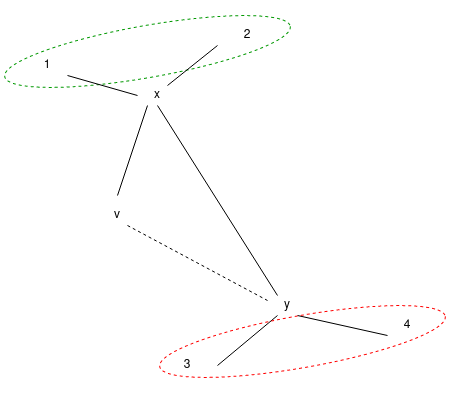
\includegraphics[scale=0.5]{images/graphs_03_03.png}
  \end{figure}
  
  We can alternatively state this condition as
  
  \bee
  d(x) + d(y) \leq n
  \eee
  
  This ensures that vertex $v$ is connected to either $x$ or $y$ but not both. Looking at the example above, we have $d(x) = 4$ and $d(y) = 3$ (not counting the dotted edge), $d(x) + d(y) \leq n = 7$, and therefore no triangle. If there were an edge $v-y$ (dotted line), we would have $d(x) = 4$ and $d(y) = 4$, $d(x) + d(y) = 8 \nleq n = 7$, and we have a triangle.

  Summing above inequality over all \emph{edges}, we find that

  \bee
  \sum_{xy \in E(G)} d(x) + d(y) \leq n e(G)
  \eee

  Instead of summing over edges, we can sum over \emph{vertices}. We do this slowly, as it took me ages to understand ;-) Let's consider a simple example first.
  
  \begin{figure}[H]
    \centering
    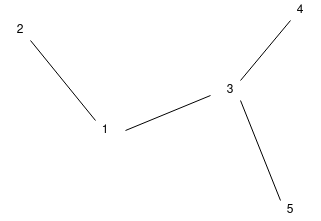
\includegraphics[scale=0.5]{images/graphs_03_04.png}
  \end{figure}
  
  We have

  \begin{align*}
  \sum_{xy \in E(G)} d(x) + d(y) & = (d(1)+ d(2)) + (d(1)+  d(3)) + (d(3) + d(4)) + (d(3) +d(5)) \\ &= 2 d(1) + d(2)+  3 d(3) + d(4) + d(5) = d^2(1) + d(2) + d^3(3) + d(4) + d(5)
  \end{align*}

  In the first equality, we have grouped the terms by edges ($1-2, 1-3, \ldots$). Generalizing, we obtain
  
  \be\label{eq:graph_03_02}
  \sum_{xy \in E(G)} d(x) + d(y) = \sum_{x \in V(G)} d^2(x) \leq ne(G)
  \ee

  We can bound the sum using Cauchy's inequality to obtain

  \bee
  \sum_{x \in G} d^2(x) \geq \frac{1}{n} \left( \sum_{x \in G} d(x) \right)^2 = \frac{1}{n} (2e(G))^2
  \eee

  where we have used \eqref{eq:graph_03:01} in the last equality. Now we use \eqref{eq:graph_03_02} to bound the left sum

  \bee
  ne(G) \geq \sum_{x \in G} d^2(x) \geq \frac{1}{n} (2e(G))^2 = \frac{4 e^2(G)}{n}
  \eee

  and we arrive at

  \bee
  e(g) \leq \frac{n^2}{4}
  \eee

\end{proof}

Given two vertices $x$ and $y$, their \emph{distance} $d(x,y)$ is the minimal length of an $x-y$-path. If there is no path between $x$ and $y$, then we set $d(x,y) = \infty$.

A graph is connected if for every distince vertex pair $x,y$, there is a path from $x$ to $y$.

A subgraph $G'$ of a graph $G$ in which any two vertices are connected to each other by paths, and which is connected to no additional vertices in the remainder of the graph $G - G'$ is a \emph{component} of the graph. A \emph{cutvertex} is a vertex whose deletion increases the number of components. Similarly, an edge is a \emph{bridge} if its deletion increases the number of components. Every vertex of a graph is contained in a unique components and an edge is a brdige if it is not contained in a cycle.

A graph without cycles is a \emph{forest} and a \emph{tree} is a connected forest. Note that a forets consists of a disjoint union of trees (I think, they need not be connected).

A \emph{bipartite} graph is a graph with two disjoint vertex classes $V_1, V_2$ where every edges connectes a vertex from set $V_1$ with a vertex from $V_2$. Note that there are no edges between vertices in $V_1$ or $V_2$. We also say that $G$ has a bipartition $(V_1, V_2)$. We can extend the concept to $r$-partite graphs with $r$ disjoint vertex classes $V_1, \ldots V_r$ and no edge joining vertices from the same vertex class. A \emph{complete $r$-partite graph} has $n_i$ vertices in the $i$-th vertex class and contains all edges joining vertices in the distinct classes. We dnote it by $K(n_1, n_2, \cdots)$; a complete bipartite graph is denoted as $K_{m,n}$ with $|V_1|=m, |V_2|=n$.

If the edges are \emph{ordered} pairs of vertices, we obtain a \emph{directed graph}. We then have directed edges $xy$ (directed from $x$ to $y$), directed paths, trails etc, and we distinguish between the \emph{outdegree} $d^+(x)$, the number of edges starting at $x$, and the \emph{indegree}, $d^-(x)$, the number of edges ending at $x$.

\subsection{Paths and Trees}

\begin{theorem}
  A graph is bipartite iff it does not contain an odd cycle.
\end{theorem}

\begin{proof}
  First we show that a bipartite graph contains even cycles: The graph $G$ has two vertex classes, $V_1, V_2$, and let the vertex sequence $x_1-x_2-x_3- \cdots - x_l$ be a cycle in $G$ (there is an edge $x_l - x_1$). Assume that $x_1 \in V_1$. Then $x_2 \in V_2, x_3 \in V_3,\ldots$; i.e. $x_i \in V_1$ iff $i$ is odd. If we consider an even cyle, then $l$ is even and therefore $x_l \in V_2$.

  Now we show that a graph without odd cycles is bipartite: Pick a vertex $x \in V(G)$ and define $V_1 = \{y: d(x,y) \text{is odd}\}$ and $V_2 = V - V_1$. There is no edge joining two vertices of the same class $V_i$, since otherwise $G$ would contain an odd cycle. Therefore $G$ is bipartite.
\end{proof}

We show the second part of the proof by means of an example graph. The left part shows the graph with vertices not separated into two sets.

  \begin{figure}[H]
    \centering
    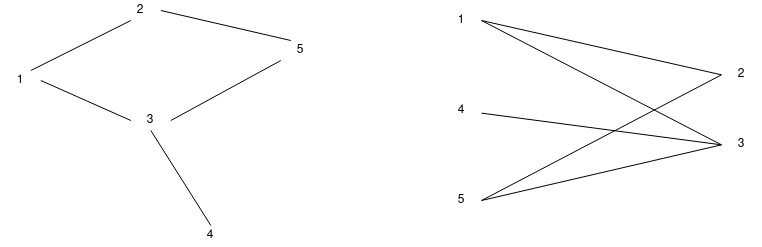
\includegraphics[scale=0.5]{images/graphs_03_05.png}
  \end{figure}

Let's choose vertex $1$ as starting point. The set $V_1$ is defined as all vertices with odd distance from $1$; therefore $V_1 = \{1, 4, 5\}$ and $V_2 = V - V_1 = \{2, 3\}$. The right part of the Figure shows the vertices of set $V_1$ on the left, the vertices of set $V_2$ on the right.

A bipartite graph has at most $|V_1| |V_2|$ edges. If we define $k = |V_1|$, the number of edges becomes $n(n-k)$. The maximum is attained in an equal distribution od vertices between the two sets; i.e. $k = n/2$ and therefore having $n(n-k) = n^2/4$ edges. This is the complete bipartite graph $K_{n/2, n/2}$.
  
\begin{theorem}
  A graph is a forest iff for every pair $\{x,y\}$ of distinct vertices it contains at most one $x-y$ path.
\end{theorem}

\begin{theorem}
  The following assertions are equivalent for a Graph $G$.
  \begin{itemize}
  \item $G$ is a tree.
  \item $G$ is a minimal connected graph: $G$ is connected, but becomes disconnected after removal of an edge $xy \in E(G)$ of $G$; i.e. $G - \{xy\}$ is disconnected. We can also say that $G$ is connected and every edge is a bridge.
  \item $G$ is a maximal acyclical graph: $G$ is acyclic (does not contain a cycle); if vertices $x$ and $y$ are nonadjacent vertices of $G$, then $G + xy$ contains a cycle.
  \end{itemize}
\end{theorem}


%%% Local Variables:
%%% mode: latex
%%% TeX-master: "journal"
%%% End:
